%-----------------------------------------------------------------------------
% Template for AIMS Structured Masters Research Project
%
% The fonts, linespacing, numbering, page styles, order
% of  Title/Abstract/TOC/Body/{Appendices}/Acknowledgements/References 
% are prescribed as the AIMS house style.
%
% Do not change them or add to it without getting approval first.
% Essays are not accepted if they do not follow house style.
% This is in preparation for your Masters where the university
% will be much more strict on the house style.
%
\documentclass{aimsessay}
\usepackage[utf8]{inputenc}
\usepackage[round]{natbib}
\usepackage{amsmath}
\usepackage{amsfonts}
\usepackage{amssymb}
\usepackage{mathtools}
\usepackage{latexsym}
\usepackage{parskip}
\usepackage{fullpage}
\usepackage{enumerate}
%
%-----------------------------------------------------------------------------
% To use external packages for specific needs, 
% get approval before adding them here (they
% should not override general AIMS house style and layout).
%
% Examples:
%
% For Arabic
\usepackage{arabtex}
\usepackage{utf8}
\setcode{utf8}
% For tables:
\usepackage{booktabs} % \toprule, \midrule, \bottomrule
\usepackage{array}    % \newcolumntype
% 
% For figures:
\usepackage[below,section]{placeins} % use \FloatBarrier in the body to really force a float somewhere. Please limit use.
% \usepackage{float}  %"H" placement spec, for **really here** (i.e. not float)
\usepackage{caption} %many figures in one figure (note subfigure and subfig are deprecated)
\usepackage{subcaption} %many figures in one figure (note subfigure and subfig are deprecated)
%
% For code and algorithms
\usepackage{moreverb}   % \verbatimtabinput
% \usepackage{listings} % more flexible and complicated 
                        % than moreverb and algorithm
% 
% Others
% \usepackage[all]{xy} 
% \usepackage{sagetex}
% \usepackage{siunitx} % to typeset numbers, units, align decimals in tables.
% \usepackage{dcolumn} % less flexible but maybe faster than siunitx above.
% \usepackage{mathtools} % More maths, e.g. \mathclap.
%
% Others may be landscape, longtable, algorithm, algorithmic, etc.
% 
% ----------------------------------------------------------------------------
% An AIMS Essay can use the sectioning commands "\chapter", "\section",
% "\subsection". No "\subsubsection", "\paragraph", etc. They are disabled.
% 
% For Theorems and such, use the environments defined here:
% \begin{thm}...\end{thm} (or "lem", "defn", etc)
% 
% We put the number to the left of the Theorem heading.
\swapnumbers 
% 
% Theorems are in italics.
\theoremstyle{plain}
\newtheorem{thm}[subsection]{Theorem}
%
% Rest is not in italics.
\theoremstyle{definition} 
\newtheorem{lem}[subsection]{Lemma}
\newtheorem{cor}[subsection]{Corollary}
\newtheorem{conj}[subsection]{Conjecture}
\newtheorem{pro}[subsection]{Proposition}
\newtheorem{exa}[subsection]{Example}
\newtheorem{defn}[subsection]{Definition}
\newtheorem{rem}[subsection]{Remark}
% 
% If you have no theorems, but a lot of equations, maybe the
% following two lines are good. Beware of corresponding Equation
% and Example numbers though! Number equations by sections.
% 
\numberwithin{equation}{section}
%
%-----------------------------------------------------------------------------
% Abstracts are usually written in English, with a version in your
% mother tongue underneath.
%
% French, Igbo, Malagasy, etc. students use normal LaTeX
% for special characters, for example \'{e}
%
% Amharic students use LibreOffice to write Amharic,
% export and include a figure.
%
%\begin{RLtext}    
%Here is where the arabic text goes.
%You can just type it with an arabic keyboard
%\end{RLtext}\\
%-----------------------------------------------------------------------------
 
% Your own command shortcuts can go here
% keep them clearly separate from other sections of the preamble
% It is good style to have only a few of these so that
% we can read one another's code. If you have to many, 
% then your code does not compile in someone else's template easily,
% and it makes it harder to read. These definitions are only
% meant for very often-used commands to save typing; Examples:
%
%\newcommand {\be}{\begin{equation}}
%\newcommand {\ee}{\end{equation}}
%\newcommand {\C}{\mathbb{C}} % Complex
%\newcommand {\Z}{\mathbb{Z}} % Integers
%\newcommand {\R}{\mathbb{R}} % Real
%\DeclareMathOperator{\sech}{sech} % declaring new math operators like \sin.
%  
%-----------------------------------------------------------------------------
% Title & Author
% On this page you must have NO full-word capitalizations, bold, or colour. 
% All AIMS research projects per year have the same title page.
% In English your family name is written last, i.e. Firstname LASTNAME
% English Capitalization, not as in some Francophone countries where
% you write LASTNAME, Firstname.
% Put your AIMS email address only please, for consistency,
% not gmail or some other webmail address.
\title{The Essay Title goes here}
% Your name must be in English Capitalisation with no comma, 
% and the Family name comes last.
\author{Firstname Middlename Familyname (email@aims.ac.za)\\
% Then in the MAIN BODY use this:                  
\begin{RLtext}    
سشمششة شمثهنعة
\end{RLtext}\\
%%%%%%%%%%%%%%%%%%%%%%%%%%%%%%%%%%%
%\begin{otherlanguage}{arabic}
%شةشىغ
%\end{otherlanguage}\\
%%%%%%%%%%%%%%%%%%%%%%%%%%%%%%%%%%%%%
% Amharic students speak to me about how to add your name in your own alphabet.
% Everything here is prescribed; do not enter bold or ALL CAPS here,
% it will not be accepted.
African Institute for Mathematical Sciences (AIMS)\\
\\
% Example1
% Supervised by Professor Barry Green
% University of Stellenbosch, South Africa
% Example2
% Supervised by Doctor Ingrid Rewitzky
% University of Stellenbosch, South Africa
{\small Supervised by: Title Firstname Lastname}\\
{\small Institute of Supervisor, Country}%
% Don't put the department, it becomes too long.
}
\date{{\small 22 May 2014}\\%
  {\scriptsize\it Submitted in partial fulfillment of 
    a structured masters degree at AIMS South Africa}\\%
  \vspace{0.5cm}{
\includegraphics{images/AIMS_Logo_square-300.jpg}}}
%-------------------------------------------------------------------------
\begin{document}
%\selectlanguage{english}
\pagestyle{empty}
\maketitle
% All other files are included via \input. 
% To compile in texmaker while viewing any of those
% without having to switch back, use
%   Options > Define Current Document as 'Master Document'
% To not have to close a PDF, remove viewpdf from quickbuild 
% and open the PDF (once) manually: it will auto-refresh or with control-r
% 
%-------------------------------------------------------------------------
% The abstract is the first thing we want to see. No acknowledgements or 
% dedications here. Fetch the abstract from a separate file.
% Please write it in English and in your mother tongue.
% An abstract should be less than half a page, so that both abstracts 
% (that is both languages) fit onto one page.
% We number roman numerals until the main body
\pagenumbering{roman}
% Abstracts are usually written in English, with a version in your
% mother tongue underneath
\chapter*{Abstract} 
\addcontentsline{toc}{chapter}{Abstract}
% Don't change anything above this.

A short, abstracted description of your research project goes here. 
It should be about 100 words long. But write it last.

An abstract is not a summary of your research project: it's an abstraction of that. 
It tells the readers why they should be interested in your research project but summarises all
they need to know if they read no further.

The writing style used in an abstract is like the style used in the rest of your research project: concise, clear and direct. 
In the rest of the research project, however, you will introduce and use technical terms. In the abstract you should
avoid them in order to make the result comprehensible to all.

You may like to repeat the abstract in your mother tongue.

% At a unviersity like Stellenbosch you *must* produce an abstract in Afrikaans for your masters.
% At AIMS you are encouraged to repeat the abstract in your mother tongue
% French, Igbo, Mlagasy, etc. just write it using LaTeX's special
% characters.
% Arabic students see the arabic.tex file for an example
% Amharic use openoffice and export from there and import a figure here.
% Where the words do not exist put the English work in italics, or use mathematical symbols.


% Do not change anything below this except for adding your
% signature (replace images/signature.png) and your name.
\vfill
\section*{Declaration}
I, the undersigned, hereby declare that the work contained in this research project is my original work, and that any work done by others or by myself previously has been acknowledged and referenced accordingly.

% Scan your signature into a small picture called 'signature.png' and insert it
% above your name and the date:
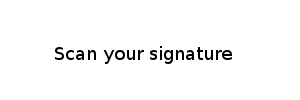
\includegraphics[height=2cm]{images/signature.png} \newline \hrule
% Your name must be in English Capitalisation with no comma, and the Family name comes last. 
% Do note the date below. It is called the "deadline".
Firstname Middlename Lastname, 27 October 2022


% Don't go typing out the contents.
\tableofcontents
\newpage
% We switch to arabic numerals here where your page count starts
% Essays must be 25-30 pages long *starting here* and up to and including
% the conclcusion. It does not include the acknowledgements or references.
% 
% Figures may differ between topics, but they are not there
% to fill the pages -- they must add meaning.
% In general most figures should be 0.8 times the width of the page
% (perhaps wider in total when two or three columns of figures)
% See the example in chapter one for defining that. Be *consistent*
% in your presentation of information.
\pagenumbering{arabic}
\pagestyle{myheadings}
%-----------------------------------------------------------------------------
% Each chapter goes in a separate file
% Chapter titles are just examples
% Always have a question
% Note the Case Pattern used at AIMS
\chapter{Introduction}

Explain the context of your essay topic, so that the
topic itself appears motivated, natural and important.

Paragraphs are separated by blank lines in the \LaTeX\ code, 
and the line spacing, paragraph indentation,
and paragraph spacing are set in the preamble for you, 
according to AIMS house style.

This is a textual citation \citet{shannon44}. And this is a parenthetical citation \citep{shannon44}.

\section{Moving On}
Let's demonstrate a figure by looking at Fig.\ \ref{bandwidth}. 

\begin{figure}[!h]
% Use "\centering" in floats (figure, table), but if you need to center
% some text (why?) use "\begin{center}...\end{center}".
\centering 
% Figure environments same as 0.8 * \textwidth please
% That does not necessarily mean the actual picture size,
% it is a guideline for the environment which could contain
% 2 or more pictures! Be consistent and follow the guidelines
% provided in your sources.
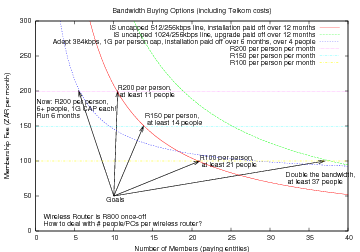
\includegraphics[width=0.8\textwidth]{images/bandwidth-colour.png}
\caption{Planning community bandwidth sharing costs. 
  Note caption capitalization.}
\label{bandwidth} 
% if you move the label it breaks the reference numbering; 
% always have it *after* the caption.
\end{figure}

Remember how to include code with {\tt verbatim} 
and to fix the tabs in {\sf python} in a verbatim environment? 
It may be best to have an `include' command for code, 
not to have to re-edit it all the time.
\verbatimtabinput{code/mycode.py}


 % Introduction is usually a chapter itself.
\chapter{The Second Chapter}

Text text text text text text text text text text text text text text
text text text text text text text text text text text text text text.

When you get stuck, don't panic. 
The world is unlikely to end just now. 
Remember you can consult your supervisor, tutor, Frances, Jan, 
and Jeff and Barry at agreed times. 

\begin{thm}[Jeff's Washing Theorem]
\label{thm:jwt}
If an item of clothing is too big, then washing it makes it bigger;
but if it is too small, washing it makes it smaller.
\end{thm}
\begin{proof}
Stated without proof. But a proof would look like this. 
\end{proof}

Notice that no Lemmas are required in the proof of Theorem \ref{thm:jwt}. % Chapters might go from 2. problem statement, 
                 % through 3. model, to 4. analysis & results
\chapter{Third Chapter}

Theorems before the chapter's first section will be dot-zero, 
and their numbering is completely wrong. You can avoid this
by simply always starting a chapter with a section. Ta Da! 
It will probably help you structure your essay anyway. 

\begin{thm}[My Theorem2]
This is my theorem2.
\end{thm}
\begin{proof}
And it has no proof2.
\end{proof}

\section{See?}

Text text text text text text text text text text text text text text
text text text text text text text text text text text text text text
text text text text text text text text text text text text text text
text text text text text text text text text text text text text text
text text text text text.

\begin{thm}[My Theorem2]
This is my theorem2.
\end{thm}
\begin{proof}
And it has no proof2.
\end{proof}

Text text text text text text text text text text text text text text
text text text text text text text text text text text text text text
text text text text text text text text text text text text text text
text text text text text text text text text text text text text text
text text text text text.

\begin{align} % do not use eqnarray. 
\label{2ya}
x & = y + y\\
\label{2yb}
& = 2y
\end{align}
see equations \ref{2ya} and \ref{2yb}

\section{More}

Here's a conjecture
\begin{conj}
The washing operation has fixed points.
\end{conj}

and here's an example

\begin{exa}
5 Rand coin.
\end{exa}


 % You do not need to have exactly 4 chapters.
                 % It is probably a good minimum, with 5 chapters 
                 % average, and 7 chapters might be a maximum.
\chapter{The Second Squared Chapter}

An average essay may contain five chapters, but I didn't plan my work properly
and then ran out of time. I spent too much time positioning my figures and worrying
about my preferred typographic style, rather than just using what was provided.
I wasted days bolding section headings and using double slash line endings, and 
had to remove them all again. I spent sleepless nights configuring manually numbered lists
to use the \LaTeX\ environments because I didn't use them from the start or understand
how to search and replace easily with texmaker.

Everyone has to take some shortcuts
at some point to meet deadlines. Time did not allow to test model 
B as well. So I'll skip right ahead and put that under my Future Work section.


\section{This is a section} 
Text text text text text text text text text text text text text text
text text text text text text text text text text text text text text
text text text text text text text text text text text text text text
text text text text text text text text text text text text text text
text text text text text. 

Some essays may have 3, 5 or 6 chapters. This is just an example. 
More importantly, do you have at most 25 pages?  
Luck has nothing to do with it. Use the techniques suggested for
writing your essay.

Now you're demonstrating pure talent and newly acquired skills. 
Perhaps some persistence. Definitely some inspiration. What was that about perspiration? 
Some team work helps, so every now and then why not browse your friends' essays and provide
some constructive feedback?
 % Conclusion is usually a chapter itself. 
%\input{chapter5} % You may have more chapters. (Use e.g. git add FILE)
% This is where we stop counting pages.
% Acknowledgements and References are not counted.
%-----------------------------------------------------------------------------
% See the acknowledgement.tex file and follow the instructions there.
\chapter*{Acknowledgements}
% Don't change anything above this.
% We do not number this or add it to the contents!
% Overly long acknowledgements are not professional.

I want to acknowledge AIMS and it's funders for the opportunity to do this work, as well as my supervisor, Prof ABC Smith from University of Hawaii.


%-----------------------------------------------------------------------------
% Note the errata page is not for now, it is for use during the examination.
% Not that you're going to have any errata.
%-----------------------------------------------------------------------------
% THE BIBLIOGRAPHY 
% Bibliography styles define how the bibliography is 
% listed and formatted. This is part of the AIMS house
% style and is only changed under exceptional circumstances
\renewcommand{\bibname}{References}
\nocite{*}
\bibliographystyle{abbrvnat}
\bibliography{references}
\addcontentsline{toc}{chapter}{References}
%-----------------------------------------------------------------------------
\end{document}
